% !TeX root = main.tex

\documentclass{article}

\usepackage{subcaption}
\usepackage[utf8]{inputenc}
\usepackage[english]{babel}
\usepackage[backend=bibtex]{biblatex}
\usepackage{tikz}
\usepackage{xcolor}
\usepackage{multicol}
\usepackage{listings}
\usepackage{csquotes}
\usepackage[most]{tcolorbox}
\usepackage{parskip}
\usepackage{listings-rust}
\usepackage[scale=0.9]{sourcecodepro}
\usepackage{bytefield}
\usepackage{tikz}
\usepackage{adjustbox}
\usepackage{float}

\addbibresource{ref}


\usetikzlibrary{arrows, automata, positioning}

\usepackage[a4paper, total={6in, 8in}]{geometry}

\tcbset {
  base/.style={
    arc=0mm,
    bottomtitle=0.5mm,
    boxsep=1mm,
    boxrule=0mm,
    colbacktitle=black!10!white,
    coltitle=black,
    fonttitle=\bfseries,
    left=2.5mm,
    leftrule=1mm,
    right=3.5mm,
    title={#1},
    toptitle=0.75mm,
  },
    sub/.style={
        base={#1},
        colframe=black!30!white,
        top=-0.5mm,
        bottom=-0.5mm,
    },
}

\definecolor{brandblue}{rgb}{0.34, 0.7, 1}
\newtcolorbox{mainbox}[1]{
    nobeforeafter,
    colframe=brandblue,
    base={#1}
}

\newtcolorbox{subbox}[1]{
  colframe=black!30!white,
  sub={#1}
}

\newtcolorbox{warningbox}[1]{
  colframe=red,
  base={#1}
}

\usepackage{lato}
\renewcommand*\familydefault{\sfdefault}
\newcommand{\code}[1]{\texttt{#1}}
\usepackage[T1]{fontenc}
\usepackage{hyperref}
\usepackage{fancyhdr}

\pagestyle{fancy}
\fancyhf{}
\rhead{Giorgio Grigolo}
\lhead{CPS 2000: Compiler Theory and Practice}
\rfoot{Page \thepage}

\definecolor{bluekeywords}{rgb}{0.13, 0.13, 1}
\definecolor{greencomments}{rgb}{0, 0.5, 0}
\definecolor{redstrings}{rgb}{0.9, 0, 0}
\definecolor{graynumbers}{rgb}{0.5, 0.5, 0.5}


\lstset{
    commentstyle=\color{greencomments},
    keywordstyle=\color{bluekeywords},
    stringstyle=\color{redstrings},
    numberstyle=\color{graynumbers},
    % breaklines=true,
    basicstyle=\ttfamily,
    language=Rust,
    xleftmargin=.3\textwidth, xrightmargin=.3\textwidth,
    captionpos=b
}

\title{Compiling \code{ParL} to \code{PArIR} in Rust \\{\normalsize A report on the Rust
compiler for the \code{ParL} programming language.}}
\author{Giorgio Grigolo - 0418803L}
\date{}

\hypersetup{
    colorlinks=true,
    linkcolor=blue,
    filecolor=magenta,
    urlcolor=blue,
}

\begin{document}

\maketitle
\tableofcontents

\vfill

\thispagestyle{empty}

\begin{abstract}
  In this report, we discuss the implementation details of a
  compiler for \code{ParL}, an expression-based strongly typed programming
  langauge. Code written in \code{ParL} is compiled to \code{PArIR}, which is
  the proprietary assembly-like language that is used to drive the
  programmable pixel art displays designed by the company \code{PArDis}. The
  \code{ParL} compiler was written in Rust, due to its strong type system and
  performance characteristics. It was implemented incrementally, as
  to ensure each component can be run in isolation, and is working correctly
  before moving on to the next one.
\end{abstract}

\vfill
\newpage
\section{Project Structure}

The \code{ParL} compiler is implemented in Rust, and is structured as a Rust
crate providing a CLI interface. The folder structure of the project reflects
the fact that the compiler was built incrementally, with each stage having the
core implementation in its own module (folder).

\subsection{Dependencies}

The use of external crate dependencies has been kept to a minimum throughout
this assignment. Currently, the only external dependencies are:

\begin{itemize}

      \item \code{clap}: A crate that provides a convenient way to define
            command-line interfaces.

      \item \code{thiserror}: A crate that provides a convenient way to define
            custom error types.

      \item \code{console}: A crate that allows for coloured printing to \code{stdout}, for decoration purposes.
\end{itemize}

\subsection{Modules}

The $\code{ParL}$ compiler is structured as a Rust crate, with the following
modules:

\begin{itemize}
      \item \code{core}: Contains the core data structures, such as the
            \code{Token} struct, the \code{TokenKind} enum and the \code{AstNode} enum,
            which are used throughout the compiler, in the majority of the stages.
      \item \code{lexing}: Contains the lexer implementation, together with its
            requirements such as the \code{Dfsa} and the \code{Lexer} struct.
      \item
            \code{parsing}: Contains the parser implementation, together with the
            \code{Parser} struct and the \code{TreePrinter} visitor.
      \item \code{semantics}: Contains a \code{visitors} folder, which
            in turn contains a number of visitors, namely the \code{SemanticAnalyser}, the \code{Formatter}, and the \code{TreePrinter}.
      \item \code{generation}: Contains the \code{ParIR} code generator visitor,
            as well as an abstraction of the \code{ParIR} language, instructions.
\end{itemize}

\newpage

\subsection{Quick Start}

The \code{ParL} compiler has a command-line tool interface, and these
are the commands that can be used to interact with. The initial run for any of
these commands will cause the Rust project to be built, so the first run might
take a bit longer than usual.

\textbf{Getting help:} $$\code{cargo run --\,-- --\,--help}$$

\textbf{Formatting a \code{ParL} file:} $$\code{cargo run fmt path/to/file.parl}$$

The above command will format the input file according to the a predetermined
style guide, and directly modify the file in place.

\textbf{Running the lexer:} $$\code{cargo run  lex path/to/file.parl}$$

The above command will print to \code{stdout} the tokens that the lexer has extracted from the input file, one per line.

\textbf{Running the parser:} $$\code{cargo run parse path/to/file.parl}$$

The above command will print to \code{stdout} the abstract syntax tree (AST)
that the parser has generated from the input file, in a pretty-printed format
provided by the \code{TreePrinter} visitor.

\textbf{Running the semantic analyser:} $$\code{cargo run sem path/to/file.parl}$$

The above command will print to \code{stdout} any semantic errors and/or warnings that the semantic analyser has found in the input file.

\textbf{Running the full compiler:} $$\code{cargo run  compile path/to/file.parl}$$

The above command will compile the input file to \code{PArIR} and print the
generated code to \code{stdout}. If the \code{-o output\_file.parir} flag is
provided, the output will be written to the specified file.

Note that all compilation related commands cause the previous steps to be run as
well, although only the output of the requested step is printed to
\code{stdout}.

\newpage

\section{Lexical Analysis}

The first step in the compilation process is the lexical analysis. A recurring
theme in the implementation of this compiler is the use of \textit{abstraction}
to achieve \textit{modularity}, and simplify the implementation of the
subsequent stages. The lexical analysis is no exception to this rule.

At the highest level, the lexical analysis is implemented as a \code{Lexer}
struct, which is responsible for reading the input source code, and producing a
stream (\textit{or vector}) of tokens.

We shall start by defining the \code{Token} struct, which is a wrapper for the
different types of tokens that can be found in a \code{ParL} program. The
\code{Token} enum is defined as follows:

\begin{mainbox}{}
    \lstset{belowskip=0pt, aboveskip=0pt}
    \begin{lstlisting}
pub struct Token {
    pub kind: TokenKind,
    pub span: TextSpan,
}
    \end{lstlisting}
\end{mainbox}

The \code{TextSpan} struct is mainly used to store the lexeme of the token, and
its position in the source code, which is useful for error reporting. The
\code{TokenKind} is just an enum, which represents the different types of tokens, such as \code{Identifier},
\code{IntegerLiteral}, \code{If} and many more.


The actual \code{Lexer} struct is defined as follows:

\begin{mainbox}{}
    \lstset{belowskip=0pt, aboveskip=0pt}
    \begin{lstlisting}[caption={The \code{Lexer} struct.}]
pub struct Lexer<B: Stream> {
    buffer: B,
    dfsa: Dfsa,
}
    \end{lstlisting}
\end{mainbox}

The \code{Lexer} struct is generic over the type \code{B}, which is a trait that
abstracts out the file reading logic from the lexer. This is useful for testing
purposes, as we can easily mock the file reading logic, and test the lexer in
isolation. It is also useful in case the lexer is to be improved in the future,
by using more efficient file reading logic, such as the double buffering
technique.

The main function of the \code{Lexer} struct is the \code{next\_token} function,
which is responsible for reading the next token from the input stream. Not much
can be said, as it has been heavily inspired by the \code{next\_token} function
in the textbook \textit{Engineering a Compiler} \cite{engineering-a-compiler}.
We provide a wrapper around the \code{next\_token} function, called
\code{lex()}, which filters out comments, whitespace and newlines, and only
returns the actual tokens, and if any, a list of errors that have been
encountered.


We note that the \code{next\_token} returns \code{Result<Token, LexicalError>}
instead of just a \code{Token}, which is caught by the wrapper \code{lex()}.
This feature, known as \textit{synchronization} allows the lexer to return an
error, instead of crashing. This enables the lexer to recover after an error has
been encountered, such as reading a character that is not in the character table
of the DFSA. It will continue reading from the next token, and find other
invalid characters.

\begin{center}
    \textit{Whilst using a compiler, one would expect to
        be given as many errors as possible, instead of
        playing whack-a-mole with the compiler.}
\end{center}

\newpage

\subsection{DFSA Builder}

Of course, the \code{Lexer} that was implemented in the project, was required to
be a based on a finite state automaton, with a character table. Initially, the
DFSA was implemented manually, but as the number of tokens (and hence states)
grew it was getting harder to keep track of the transitions.

To solve this problem, together with the \code{Dfsa} struct, a
\code{DfsaBuilder} struct was implemented, which is responsible for dynamically
building the DFSA from a number of chained function calls. I will describe each
method of the \code{DfsaBuilder} struct, and how it is used, by demonstrating
the effect as it is run incrementally on an empty DFSA.


The \code{DfsaBuilder} struct is defined as follows:

\begin{mainbox}{}
    \lstset{xleftmargin=0cm}
    \begin{lstlisting}
pub struct DfsaBuilder {
    pub max_state: i32,
    pub accepted_states: Vec<i32>,
    pub character_table: HashMap<char, Category>,
    pub transition_table: HashMap<(i32, Category), i32>,
    pub state_to_token: HashMap<i32, TokenKind>,
}
    \end{lstlisting}
\end{mainbox}

Clearly, we can see that states are represented by \code{i32} integers, and
transitions are represented by a tuple of the current state and the category of
the character that is being read. The category of a character is defined by the
\code{Category} enum, containing variants such as \code{Digit}, \code{Letter},
\code{Whitespace}, and many more.


The first function is $$\code{add\_category(\&mut self, range: Vec<char>,
        category: Category)}$$  This method is used to add multiple characters to the
same category.  For example, we can add all the digits to the \code{Digit}
category, by calling \code{add\_category('0'..='9', Category::Digit)}. Note that
in the actual implementation, the \code{range} parameter is actually a more
complex type, but for simplicity's sake it can be thought of a vector. It
actually accepts anything that can be casted to an iterator, as to allow for
more convenient usage. This is done using Rust's built in ranges like
\code{'0'..='9'}. As it does not have any effect on the DFSA, but only modifies
the character table, a DFSA will not be shown.

Then, we have $$\code{add\_transition(\&mut self, state: i32, category:
        Category, next\_state: i32)}$$ This method is used to add a transition from one
state to another, given a category. For example, we can add a transition from
state 0 to state 1, when reading a digit, by calling \code{add\_transition(0,
    Category::Digit, 1)}. Note that it doesn't automatically make the state 1 an
accepted state, as it is only responsible for adding transitions.


\begin{figure}[H]
    \begin{subfigure}[t]{0.5\textwidth}
        \centering
        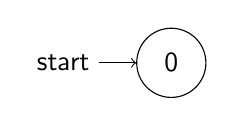
\begin{tikzpicture}
            \node[state, initial] (0) {0};
        \end{tikzpicture}
        \caption{The DFSA before adding calling \code{add\_transition}}
    \end{subfigure}
    \begin{subfigure}[t]{0.5\textwidth}
        \centering
        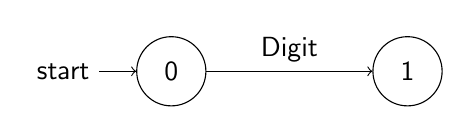
\begin{tikzpicture}
            \node[state, initial] (0) {0};
            \node[state, right of=0, xshift=2cm] (1) {1};
            \draw (0) edge[above, ->] node{Digit} (1);
        \end{tikzpicture}

        \caption{The DFSA after adding calling \code{add\_transition}}
    \end{subfigure}
\end{figure}

The next function is $$\code{auto\_add\_transition(\&mut self, state: i32,
        category: Category}$$
$$\code{to: Option<i32>, token\_kind: TokenKind) -> i32}$$

This method is used used to add a transition from \code{(state, category)} to
the state \code{to}. Since \code{to} is an \code{Option}, it can be \code{None},
in which case the destination state is automatically set to the next state. This
is useful for adding transitions to the same state, as well as constructing
slightly more complicated sequences of transitions, say for tokenizing a float.
The \code{token\_kind} parameter is used to set the token kind of the state, if
it is an accepted state. Similarly to the \code{to} parameter, it can be
\code{None}, in which case the destination state is not an accepted state.  We
also note that this function returns an integer, which is the state that was
just added, for further use in subsequent calls.

If we run \code{auto\_add\_transition(2, Category::Digit, None, Category::Float)}, the resultant DFSA will be as follows:

\begin{figure}[H]
    \begin{subfigure}[t]{0.5\textwidth}
        \centering
        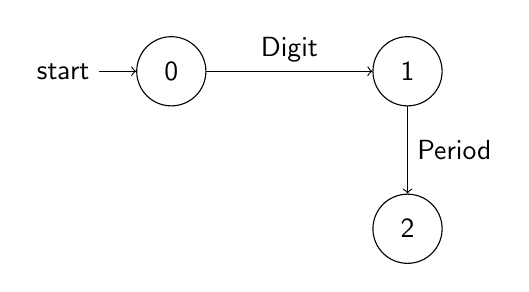
\begin{tikzpicture}
            \node[state, initial] (0) {0};
            \node[state, right of=0, xshift=2cm] (1) {1};
            \node[state, below of=1, yshift=-1cm] (2) {2};

            \draw (0) edge[above, ->] node{Digit} (1)
            (1) edge[right, ->] node{Period} (2);
        \end{tikzpicture}
        \caption{Before running the function}
    \end{subfigure}
    \begin{subfigure}[t]{0.5\textwidth}
        \centering
        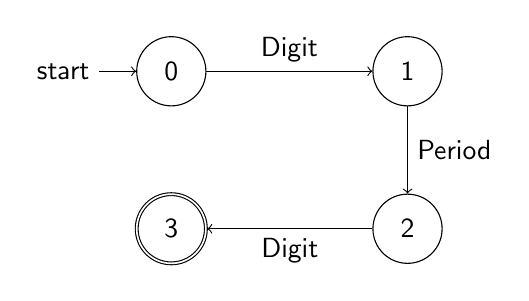
\begin{tikzpicture}
            \node[state, initial] (0) {0};
            \node[state, right of=0, xshift=2cm] (1) {1};
            \node[state, below of=1, yshift=-1cm] (2) {2};
            \node[state, accepting, below of=0, yshift=-1cm] (3) {3};

            \draw (0) edge[above, ->] node{Digit} (1)
            (1) edge[right, ->] node{Period} (2)
            (2) edge[below, ->] node{Digit} (3);
        \end{tikzpicture}
        \caption{After running the function}
    \end{subfigure}
\end{figure}

If we run \code{auto\_add\_transition(2, Category::Digit, Some(5), None)}, the
resultant DFSA will be as follows, meaning we just want to map to an auxiliary
state that doesn't correspond to any token kind, (and thus is not an accepted
state), the following is the resulting DFSA.

\begin{figure}[H]
    \begin{subfigure}[t]{0.5\textwidth}
        \centering
        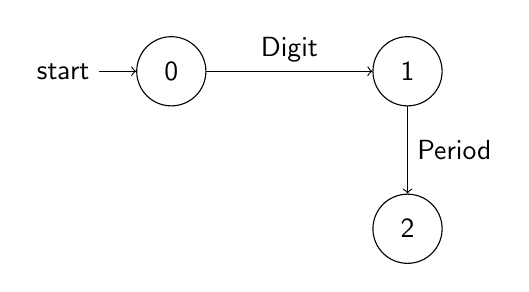
\begin{tikzpicture}
            \node[state, initial] (0) {0};
            \node[state, right of=0, xshift=2cm] (1) {1};
            \node[state, below of=1, yshift=-1cm] (2) {2};

            \draw (0) edge[above, ->] node{Digit} (1)
            (1) edge[right, ->] node{Period} (2);
        \end{tikzpicture}
    \end{subfigure}
    \begin{subfigure}[t]{0.5\textwidth}
        \centering
        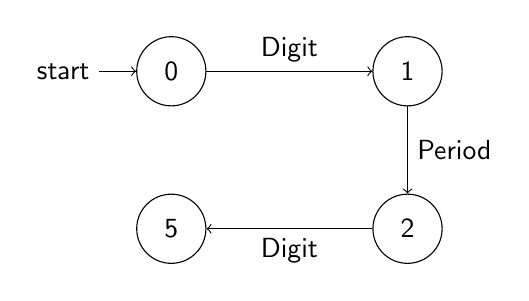
\begin{tikzpicture}
            \node[state, initial] (0) {0};
            \node[state, right of=0, xshift=2cm] (1) {1};
            \node[state, below of=1, yshift=-1cm] (2) {2};
            \node[state, below of=0, yshift=-1cm] (3) {5};

            \draw (0) edge[above, ->] node{Digit} (1)
            (1) edge[right, ->] node{Period} (2)
            (2) edge[below, ->] node{Digit} (3);

        \end{tikzpicture}
    \end{subfigure}
\end{figure}

Next up, we have the function

\begin{center}
    \code{add\_final\_character\_symbol(character: char, category: Category, token\_kind: TokenKind)}
\end{center}

This function is a shortcut for adding single characters that are final symbols,
such as the semicolon, or the period to the character table, and the transition
that follows from this to the transitions table.

Suppose we called \code{add\_final\_character\_symbol(';',
    Category::Semicolon,} \\ \code{TokenKind::Semicolon)}. The resultant DFSA would
be as follows:

\begin{figure}[H]
    \begin{subfigure}[t]{0.5\textwidth}
        \centering
        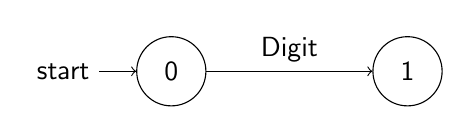
\begin{tikzpicture}
            \node[state, initial] (0) {0};
            \node[state, right of=0, xshift=2cm] (1) {1};

            \draw (0) edge[above, ->] node{Digit} (1);
        \end{tikzpicture}
    \end{subfigure}
    \begin{subfigure}[t]{0.5\textwidth}
        \centering
        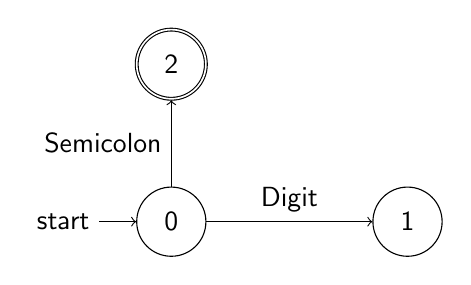
\begin{tikzpicture}
            \node[state, initial] (0) {0};
            \node[state, right of=0, xshift=2cm] (1) {1};
            \node[state, accepting, above of=0, yshift=1cm] (2) {2};

            \draw (0) edge[above, ->] node{Digit} (1)
            (0) edge[left, ->] node{Semicolon} (2);
        \end{tikzpicture}
    \end{subfigure}
\end{figure}

Then we have a function that does the same thing as the previous one, but is
able to take in multiple tuples of the type (\code{char}, \code{Category},
\code{TokenKind}), and add them all at once. This function is called
\code{add\_final\_character\_symbols}.

Finally, we have the function \code{build}, which is used to build the DFSA from the builder. This function is called at the end of the chain of function calls, and returns the DFSA that was built.

\begin{center}
    \rule{0.5\textwidth}{0.4pt}
\end{center}

Clearly, the \code{DfsaBuilder} has proved itself useful for an efficient and
readable way to build the DFSA for the lexer. However, we still require a
greater degree of freedom when it comes to making complex multi-character
transitions.

\begin{warningbox}{}
    In the production rules for the \code{ParL} grammar, there is a slight
    inconsistency. There is an overlap between the \code{Letter} and the
    \code{Hex} symbol. This was taken into account by creating an auxiliary
    category called \code{HexAndLetter}, so that the lexer can differentiate
    between the two.
\end{warningbox}

To be able to get around the above inconsistency, as well as to allow for the
aforementioned flexibility, we can also call the \code{.transition()} method on
the \code{DfsaBuilder}, and have it return an instance of the \code{Transition}
struct. This transition automatically starts from the first unused state index,
(which is kept track of in the \code{max\_state} member of the
\code{DfsaBuilder} struct) and gives us another set of functions we can chain to
further build the transition.

The \code{Transition} struct holds a reference to the \code{DfsaBuilder} that it
was created from, the current state, the list of transitions that have been
added, and the a list of final states with the token kind that they return.

\begin{mainbox}{}
    \lstset{xleftmargin=1cm}
    \begin{lstlisting}
pub struct Transition<'a> {
    dfsa_builder: &'a mut DfsaBuilder,
    current_state: i32,
    transitions: Vec<((Category, i32), i32)>,
    final_state_token: Vec<(i32, TokenKind)>,
}
    \end{lstlisting}
\end{mainbox}


The first function that can be called on the \code{Transition} struct is the following:
$$\code{to(category: Category) -> Transition}$$

This method is used to just append a single category to the transition. Calling
it multiple times, increments an internal pointer, that always points to the
last state that was added. Thus, calling it multiple times creates a
\textit{chain} of states.


\begin{figure}[H]
    \begin{subfigure}[t]{0.5\textwidth}
        \centering
        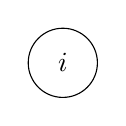
\begin{tikzpicture}
            \node[state] (0) {$i$};
        \end{tikzpicture}
        \caption{The transition before adding calling \code{to}}
    \end{subfigure}
    \begin{subfigure}[t]{0.5\textwidth}
        \centering
        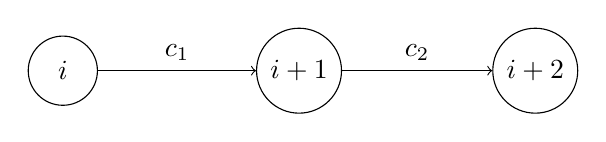
\begin{tikzpicture}
            \node[state] (0) {$i$};
            \node[state, right of=0, xshift=2cm] (1) {$i+1$};
            \node[state, right of=1, xshift=2cm] (2) {$i+2$};
            \draw (0) edge[above, ->] node{$c_1$} (1);
            \draw (1) edge[above, ->] node{$c_2$} (2);
        \end{tikzpicture}
        \caption{The transition after adding calling \code{to} twice with $c_1$ and $c_2$ respectively}
    \end{subfigure}
\end{figure}


Then, we have the $\code{repeated()}$ method, which is used to allow an
indeterminate number of repetitions of the last category, think of this as the
\code{*} symbol in regular expressions.

\begin{figure}[H]
    \begin{subfigure}[t]{0.5\textwidth}
        \centering
        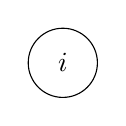
\begin{tikzpicture}
            \node[state] (0) {$i$};
        \end{tikzpicture}
        \caption{The transition before adding calling \code{repeated}}
    \end{subfigure}
    \begin{subfigure}[t]{0.5\textwidth}
        \centering
        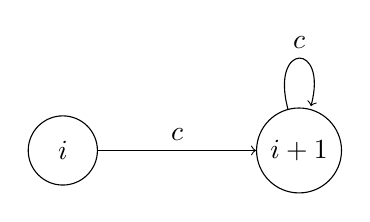
\begin{tikzpicture}
            \node[state] (0) {$i$};
            \node[state, right of=0, xshift=2cm] (1) {$i+1$};
            \draw (0) edge[above, ->] node{$c$} (1);
            \draw (1) edge[above, ->, loop above] node{$c$} (1);
        \end{tikzpicture}
        \caption{The transition after adding calling \code{to(c)} followed by  \code{repeated()}}
    \end{subfigure}
\end{figure}


Whenever we want to make the last state an accepted state, we can thenc all the
$$\code{goes\_to(token\_kind: TokenKind)}$$ method, that simply marks the last state as
an accepted state, and sets the token kind it returns to the one that was passed
as an argument.

Finally, we have the $\code{done()}$ method, which is used to append the transition that has been prepared to the actual DFSA from which \code{.transition()} was called from.


\begin{mainbox}{Full example}
    \lstset{xleftmargin=1cm, aboveskip=0pt, belowskip=0pt}
    \begin{lstlisting}
        let mut builder = DfsaBuilder::new();
        builder.add_category([' '], ['\t'], Category::Whitespace)
               .transition()
               .to([Category::Whitespace])
               .repeated()
               .goes_to(TokenKind::Whitespace)
               .done();
    \end{lstlisting}
\end{mainbox}

Would result in the following DFSA, with the category table already filled in
with the whitespace characters.

\begin{figure}[H]
    \centering
    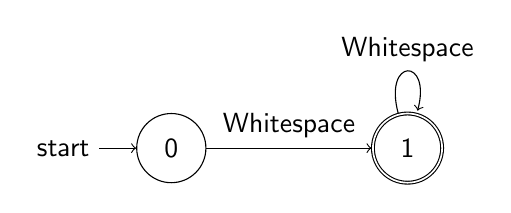
\begin{tikzpicture}
        \node[state, initial] (0) {0};
        \node[state, accepting, right of=0, xshift=2cm] (1) {1};

        \draw (0) edge[above, ->] node{Whitespace} (1);
        \draw (1) edge[above, ->, loop above] node{Whitespace} (1);
    \end{tikzpicture}
\end{figure}

The actual definitions of the DFSA that was used in the lexer can be found in
\code{lexer.rs}, as part of the \code{Lexer::new()} function, and also in
Appendix \ref{sec:lexer-dfsa}. The final thing I must mention is how keyword are
interpreted. Keywords are treated as identifiers, and then checked against a
\code{HashMap} of reserved keywords. If the identifier is found in the map, the
token kind is changed to the corresponding keyword.
% \newpage

\section{Parsing the Token Stream}

Parsing the token stream generated by the lexer is where the Rust language
really shines. It allows to define an enum, called \code{AstNode}, which
represents the different types of nodes that can be found in the abstract syntax
tree of a \code{ParL} program. Additionally, we can mix and match different
types of variants, such as ones with no data (similar to unit-like structs, like
\code{struct Foo;}), ones with unnamed data (similar to tuple structs, like
\code{struct Foo(i32, i32);}), and ones with named data (similar to regular
structs, like \code{struct Foo \{ x: i32, y: i32 \};}).

This gives us much more flexibility when defining the AST, in contrast to C or
C++, where enums are basically just integers. Furthermore, I had to create a
type alias from \code{Box<AstNode>} to \code{AstNodePtr}. This is because
certain \code{AstNode} variants, have another \code{AstNode} as a child. The
Rust compiler complains about the enum having infinite size, as it is can't be
calculated at compile time. This is understandable, as for example, if the
\code{AstNode::Expression} variant contained another \code{AstNode} as its
member, the compiler would try to recursively visit this member to check its
size, which could also be an expression, visiting the same member again, and so
on. With a \code{Box}, the size of the enum is known at compile time, as it is
just a pointer to the heap, and the compiler is happy. Lists of \code{AstNode}s,
like parameter lists, do not need this, as a Rust \code{Vec} is already
allocated on the heap.

The actual parser is implemented as a struct called \code{Parser}, which must be
initialized with the list of tokens generated by the lexer. The parser privately
defines all the different parsing functions. The only public function is
\code{parse}, which is called to start the parsing process. The parser uses a
recursive descent parsing algorithm, together with the Rust pattern matching
feature, which is used to differentiate between the different variants of the
\code{AstNode} enum.

Due to this, the Visitor design pattern is slightly different in Rust. With
pattern matching, we avoid having every variant of the \code{AstNode} enum
requiring it's own \code{accept} method. Instead we define each case in the
\code{match} clause in the \code{visit} method for a given struct implementing
the \code{Visitor} trait. Pattern matching is thoroughly used to ensure
correctness and to avoid unnecessary code duplication.

A number of utility functions, such as \code{consume\_if(kind:\,Tokenind)}, and
\code{assert\_token\_is\_any}\\\code{(kind:\ Vec<TokenKind>)}, are used to
simplify the parsing process. The former consumes a token if it matches the
given \code{TokenKind}, and returns an error otherwise. This is useful as it in
allows the user to quickly identify syntax errors in the input program, with the
parser suggesting what it was expecting, and announcing what it found instead.
The latter function, asserts that the current token is any of the given
\code{TokenKind}s, and returns an error if it is not. This is useful when the
parser is expecting one of a number of different tokens, such as when declaring
a variable, we expect either an \code{int}, \code{float}, \code{colour} or
\code{bool} token kind after the semicolon. The error outputted will be more
informative, as it will list all the possible token kinds that were expected.

The full list of the \code{AstNode} enum variants can be found in Appendix
\ref{sec:parser-ast-node-enum}.
\newpage
\section{Semantic Analysis}
\newpage
\section{Code Generation}

The final step in the compilation process is the code generation phase. In this phase, the compiler takes the AST and generates the \code{PArIR} code that will be executed by the \code{PArDis} displays.

\subsection{Abstracting Instructions}

The first step in the code generation phase was to abstract the \code{PArIR}
instructions into a Rust enum. This enum, called \code{Instruction}, contains
all the instructions that the \code{PArDis} displays can execute. Some of the
instructions, like \code{Push}, \code{Pusha} and really most of the push
variants, take some arguments, which are stored in the enum itself, as an
unnamed tuple e.g. \code{PushValue(usize)}.

The \code{Instruction} enum has a \code{Display} trait implementation, which is
equivalent to a \code{toString} method in other languages. We will set the
string representation of the instruction to be the same as the \code{PArIR}
instruction itself, with the arguments formatted accordingly, as it will be
outputted in the final \code{PArIR} code.

\subsection{Program Intermediate Representation}

Fundamentally, we can represent a \code{PArIR} program as an ordered list of
instructions. Furthermore, these instructions can be grouped in two sections:
\begin{itemize}
    \item The \textit{function section}, which contains all the function definitions.
    \item The \textit{main section}, the entrypoint of the program, which
          contains the instructions that will be executed when the program starts.
\end{itemize}

In fact, our \code{Program} struct, is exactly the above.

\begin{mainbox}{}
    \lstset{xleftmargin=.2\textwidth, aboveskip=0pt, belowskip=0pt}
    \begin{lstlisting}
struct Program {
    pub functions: Vec<Instruction>,
    pub main: Vec<Instruction>,
}
\end{lstlisting}
\end{mainbox}

When writing the resulting \code{PArIR} code to a file, we first write the
function section, followed by the main section. Due to the fact that the only
thing we need to call a function, is its name, not the line number where it has
been defined, we can successfully divide the program into these two sections.

\newpage

\subsection{Code Generation Visitor}

The code generation visitor is the final visitor that is run on the AST.
Contrary to the the semantic analyser, instead of returning type information as
it visits the nodes of the AST, it returns \textit{line numbers} of the
generated \code{PArIR} code. These line numbers are mostly used to generate all
kinds \code{Jump} instructions correctly. For example, when we generate an if
statement, we need to know the line number of the first instruction of the true
branch, and that of the false branch, so that upon evaluating the condition, we
know where to jump.

Of course, other things need to be kept track of, like the current stack level,
and the current frame index, which are used to generate the correct \code{Push}
instructions when referencing variables from the symbol table. Here is the full
definition of the \code{PArIRWriter} struct, upon which we implement the visitor
trait.

\begin{mainbox}{}
    \lstset{xleftmargin=.1\textwidth, aboveskip=0pt, belowskip=0pt}
    \begin{lstlisting}
pub struct PArIRWriter {
        /// Stack of symbol tables, each representing a scope
        symbol_table: Vec<SymbolTable>,
        /// The ParIR program container
        program: Program,
        /// Pointer to the current instruction
        instr_ptr: usize,
        /// The current stack level
        stack_level: usize,
        /// The current frame index
        frame_index: usize,
    }
\end{lstlisting}
\end{mainbox}

Additionally, we also have some helper functions such as

\begin{itemize}
    \item \code{get\_scope\_var\_count}, which returns the number of slots in
          the that we need to allocate in the stack frame for the current scope.
    \item \code{get\_memory\_location(token: Token)}, which returns the memory
          location of a variable, given its name.  \item \code{push\_scope()} and
          \code{pop\_scope()}, being common operations, we shall automate them, whilst
          resetting the frame index and incrementing the stack level.
\end{itemize}


\newpage

\section{Arrays}

Implementing arrays was definetely a challenge that required a lot of thought,
and changes in previous parts of the codebase. Some of the AST nodes needed to
store some extra information, and thus the parser had to be partially revisited.

\subsection{Parser Changes}

Although functional, array usage is quite restricted. For example, due to the
definition of the grammar, expressions arent't allowed to be used as array elements. In other words, the following
variable declaration would be syntactically incorrect:

$$ \code{let a: int[4] = [1+2, 3, 4, 5];} $$

The reason for this is that the grammar doesn't allow for expressions to be used
as array elements. This is a limitation that could be easily fixed by adding a
new rule to the grammar, but it was decided to leave it as is for the sake of
simplicity.

Furthermore, it was noted that unlike \code{Int}s, \code{Bool}s, \code{Colour}s
and \code{Float}s, the grammar doesn't offer a \code{Literal} variant for arrays.
In a function declaration, this would again be syntactically incorrect:

{\lstset{xleftmargin=0.25\textwidth}
\begin{lstlisting}
fun rot_arr() -> int[4] {
    let a: int[4] = [1, 2, 3, 4];
    return [a[1], a[2], a[3], a[0]];
}
\end{lstlisting}}

\subsection{Semantic Analysis Changes}

The semantic analysis was also updated to support arrays. The new type variant
in the \code{Type} enum $$\code{Array(Box<Type>, usize)}$$ was introduced to
represent arrays. Note that in a similar fashion to the \code{AstNode} enum, we
have to wrap the type in a \code{Box} to avoid infinite size of the \code{Type}
enum. Theoretically, this would allow the support for multi-dimensional arrays
in our type system, but that would require massive changes starting again from
the parser.

This changes allows us to hook up the type checker seamlessly, to ensure that
when arrays are passed to functions as parameters, these are checked to be of
the same type and size as the expected parameter.

\subsection{Code Generation Changes}

The code generation was also updated to support arrays. The main changes
consisted of adding the new instructions, namely \code{StoreArray},
\code{PushArray(MemoryLocation)}, \code{PushOffsetFromOpS(MemoryLocation)},
\code{PrintArray} and \code{ReturnArray}. The latter however, although available
as instruction in the VM, was not used. Even though clearly, we have seen that
functions can return arrays (although they have to be declared temporarily
inside and mutated only through direct array accesses), a slight workaround has
been implemented to achieve \textbf{properly ordered} that happens to fix other
issues that arise when referencing arrays. It was noted that some VM
instructions are inconsistent with the ordering in the storage and loading of
arrays from the operand stack.

Thus, when traversing the AST and finding an identifier which points to an
array, the following workaround occurs.
\graphicspath{figures}

\begin{figure}[H]
    \centering
    \begin{subfigure}{.5\textwidth}
        \centering
        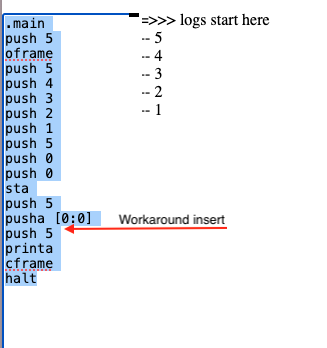
\includegraphics[width=0.6\textwidth]{figures/no_wk.png}
        \caption{Array printing without the workaround}
        \label{fig:no_wk}
    \end{subfigure}%
    \begin{subfigure}{.5\textwidth}
        \centering
        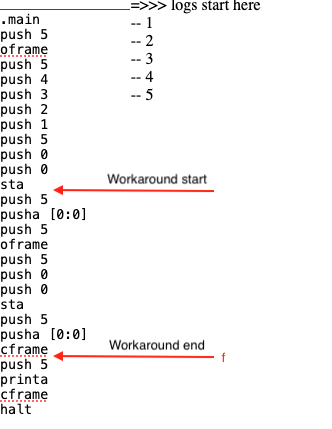
\includegraphics[width=0.5\textwidth]{figures/image.png}
        \caption{Array printing with the workaround}
        \label{fig:array_print}
    \end{subfigure}
    \caption{Inconsistent pusha and printa behaviour}
    \label{fig:array_instructions}
\end{figure}


In essence, when we find an identifier that points to an array, and call
\code{PushArray}, the contents of the array are actually pushed in reverse
order. Calling \code{PrintArray} reveals this. The workaround consists of
creating a new temporary frame with as much space as the array size, and then
store the array in the frame. Subsequently the array is pushed back to the
operand stack, but this time in the correct order. The frame is then closed and
code generation continues as usual.

Like this, wherever we use arrays, we have the guarantee that the array is
pushed in the correct order, and that it can be used anywhere as expected, even
when accessing it.



\newpage

\section{Testing Framework}

\subsection{Unit Testing}

During the early stages of development, such as the lexer and parser, most of
the testing was done through unit tests, first with smaller cases, and then with
larger cases.

\subsection{Integration Testing}

After the lexer and parser were completed, integration testing was done to
ensure that the lexer and parser worked together correctly. This was done by
running the CLI interfce, one stage at a time, on small, simple prorgrams.

Nearing the end of the project, I decided that it would be useful to create a
more robust testing framework to test the entire compiler, as well as the
compiled code on the VM. Using the Python library
\href{https://playwright.dev/python/}{Playwright} I created a script that opens
the VM website in a browser (in headless mode) and runs the compiled code. The
script then gets the output of the log, transforms it into an array of its
lines, and removes the three \code{`>'} symbols at the beginning of each log
entry.

In Python then, we are free to use this array to check against the expected
values, through assertions, and we print out the results of the tests.



\subsection{Results}

\subsubsection{Variable declarations}

\textbf{ParL Program:}

\begin{lstlisting}
    let a: int = 5;
    let b: colour = #000000;
    let c: float  = 1.23;

    let d: int[5] = [1, 2, 3, 4, 5];

    __print a;
    __print b;
    __print c;
    __print d;

    {
        let a: int = 1;
        __print a;
    }

    __print a;
\end{lstlisting}

\newpage

\textbf{AST:}

\begin{lstlisting}
Program
  VarDec
    Identifier: a
    Type: int
    Expression: 5
  VarDec
    Identifier: b
    Type: colour
    Expression: #000000
  VarDec
    Identifier: c
    Type: float
    Expression: 1.23
  VarDecArray
    Identifier: d
    Element Type: int
    Size: 5
    Elements: 1, 2, 3, 4, 5
  Print
    Expression: a
  Print
    Expression: b
  Print
    Expression: c
  Print
    Expression: d
  Block
    VarDec
      Identifier: a
      Type: int
      Expression: 1
    Print
      Expression: a
  Print
    Expression: a
\end{lstlisting}

\textbf{Result:}
Output successfuly matched with $$\code{['5', '0', '1.23', '1', '2', '3', '4',
                '5', '1', '5']}$$

\newpage

\subsubsection{Variable Assignment}

\textbf{ParL Program:}

\vfill

\begin{lstlisting}
    let a: int = 5;
    let b: colour = #000000;
    let c: float  = 1.23;
    let d: int[5] = [1, 2, 3, 4, 5];

    __print a;
    __print b;
    __print c;
    __print d[1];

    a = 2;
    b = #FFFFFF;
    c = 3.45;
    d[1] = 1;

    __print a;
    __print b;
    __print c;
    __print d[0];
\end{lstlisting}
\vfill

\newpage

\textbf{AST:}


\begin{lstlisting}[language=]
Program
  VarDec
    Identifier: a
    Type: int
    Expression: 5
  VarDec
    Identifier: b
    Type: colour
    Expression: #000000
  VarDec
    Identifier: c
    Type: float
    Expression: 1.23
  VarDecArray
    Identifier: d
    Element Type: int
    Size: 5
    Elements: 1, 2, 3, 4, 5
  Print
    Expression: a
  Print
    Expression: b
  Print
    Expression: c
  Print
    Expression: ArrayAccess
        Identifier: d
        Index: 1
  Assignment
    Identifier: a
    Expression: 2
  Assignment
    Identifier: b
    Expression: #FFFFFF
  Assignment
    Identifier: c
    Expression: 3.45
  Assignment
    Identifier: d
    Expression: 1
    Index: 1
  Print
    Expression: a
  Print
    Expression: b
  Print
    Expression: c
  Print
    Expression: ArrayAccess
        Identifier: d
        Index: 0
\end{lstlisting}


\textbf{Result:}

Output successfuly matched with $$\code{["5", "0", "1.23", "2", "2", "16777215",
                "3.45", "1"]}$$


\subsubsection{Control Flows}

\textbf{ParL Program:}

{

    \lstset{xleftmargin=0.2\textwidth}

    \begin{lstlisting}
    let loop_max: int = 5;

    for (let i: int = 0; i < loop_max; i = i + 1) {
        __print i;
    }

    if (1 < 2) {
        __print 1;
    } else {
        __print 0;
    }

    if (1 > 2) {
        __print 1;
    } else {
        __print 0;
    }


    let i: int = 0;
    while (i < loop_max) {
        __print i;
        i = i + 1;
    }
\end{lstlisting}

}

\newpage

\textbf{AST:}


\begin{lstlisting}
Program
  VarDec
    Identifier: a
    Type: int
    Expression: 5
  VarDec
    Identifier: b
    Type: colour
    Expression: #000000
  VarDec
    Identifier: c
    Type: float
    Expression: 1.23
  VarDecArray
    Identifier: d
    Element Type: int
    Size: 5
    Elements:
      1, 2, 3, 4, 5,
  Print
    Expression: a
  Print
    Expression: b
  Print
    Expression: c
  Print
    Expression: ArrayAccess
        Identifier: d
        Index: 1
  Assignment
    Identifier: a
    Expression: 2
  Assignment
    Identifier: b
    Expression: #FFFFFF
  Assignment
    Identifier: c
    Expression: 3.45
  Assignment
    Identifier: d
    Expression: 1
    Index: 1
  Print
    Expression: a
  Print
    Expression: b
  Print
    Expression: c
  Print
    Expression: ArrayAccess
        Identifier: d
        Index: 0
\end{lstlisting}

\textbf{Result:}

Output successfuly matched with $$\code{["0", "1", "2", "3", "4", "1", "0", "0", "1", "2", "3", "4"]}$$

\newpage

\subsubsection{Functions}

\textbf{ParL Program:}
{
    \lstset{xleftmargin=0.2\textwidth}

    \begin{lstlisting}
fun add(a: int, b: int) -> int {
    return a + b;
}

let result: int = add(5, 10);

__print result;

fun some_func(a: int[2]) -> int[2] {
    let b: int[2] = [1,3];
    return b;
}

let a: int[2] = [1, 2];

__print some_func(a);


fun mixed_parameters(a: int, b: float, c: colour) -> bool {
    __print a;
    __print b;
    __print c;

    return true;
}

__print mixed_parameters(5, 1.23, #000000);

fun array_parameters(a: int[5]) -> int {

    let sum: int = 0;

    for (let i: int = 0; i < 5; i = i + 1) {
        __print a[i];
        sum = sum + a[i];
    }

    return sum;
}

let arr: int[5] = [5, 1, 2, 3, 4];

__print array_parameters(arr);

\end{lstlisting}
}

\newpage

\textbf{AST:}

{

    \lstset{xleftmargin=0.25\textwidth}

    \begin{lstlisting}
Program
  FunctionDecl
    Identifier: add
    Params: a: int, b: int,
    Return Type: int
    Block: Block
      Return
        Expression: (a + b)
  VarDec
    Identifier: result
    Type: int
    Expression: add(5, 10)
  Print
    Expression: result
  FunctionDecl
    Identifier: some_func
    Params: a: int[2],
    Return Type: int[2]
    Block: Block
      VarDecArray
        Identifier: b
        Element Type: int
        Size: 2
        Elements:
          1, 3,
      Return
        Expression: b
  VarDecArray
    Identifier: a
    Element Type: int
    Size: 2
    Elements:
      1, 2,
  Print
    Expression: some_func(a)
  FunctionDecl
    Identifier: mixed_parameters
    Params: a: int, b: float, c: colour,
    Return Type: bool
    Block: Block
      Print
        Expression: a
      Print
        Expression: b
      Print
        Expression: c
      Return
        Expression: true
  Print
    Expression: mixed_parameters(5, 1.23, #000000)
  FunctionDecl
    Identifier: array_parameters
    Params: a: int[5],
    Return Type: int
    Block: Block
      VarDec
        Identifier: sum
        Type: int
        Expression: 0
      For
        Initializer: VarDec
          Identifier: i
          Type: int
          Expression: 0
        Condition: (i < 5)
        Increment:
          Assignment
            Identifier: i
            Expression: (i + 1)

        Body: Block
          Print
            Expression: ArrayAccess
                Identifier: a
                Index: i
          Assignment
            Identifier: sum
            Expression: (sum + ArrayAccess
                Identifier: a
                Index: i)
      Return
        Expression: sum
  VarDecArray
    Identifier: arr
    Element Type: int
    Size: 5
    Elements:
      5, 1, 2, 3, 4,
  Print
    Expression: array_parameters(arr)
\end{lstlisting}

}

\textbf{Result:}

Output successfuly matched with $$\code{["15", "1", "3", "5", "1.23", "0", "1",
                "5", "1", "2", "3", "4", "15"]}$$

\newpage

\subsubsection{Expressions}

\textbf{ParL Program:}

{
    \lstset{xleftmargin=0.1\textwidth}

    \begin{lstlisting}
let a: int = 5;
let b: int = 10;

__print (a + b) == 20;
__print ((((a + b) * 2) / 3) - 1) == 9;
__print (a + b) <= 20 and a - b <= 0;
__print ((12 + 5) * (8 - 3) + (18 / 2)) - ((25 - 5) / (4 + 1));
\end{lstlisting}

}

\textbf{AST:}

{

    \lstset{xleftmargin=0\textwidth}

    \begin{lstlisting}
Program
  VarDec
    Identifier: a
    Type: int
    Expression: 5
  VarDec
    Identifier: b
    Type: int
    Expression: 10
  Print
    Expression: (((a + b)) == 20)
  Print
    Expression: (((((((((a + b)) * 2)) / 3)) - 1)) == 9)
  Print
    Expression: ((((a + b)) <= 20) and ((a - b) <= 0))
  Print
    Expression: ((((((12 + 5)) * ((8 - 3))) + ((18 / 2)))) - ((((25 - 5)) / ((4 + 1)))))
\end{lstlisting}

}

\textbf{Result:}

Output successfuly matched with $$\code{["0", "1", "1", "90"]}$$

\newpage

\subsubsection{Pad Read/Write}

\textbf{ParL Program:}

{
    \lstset{xleftmargin=0.2\textwidth}

    \begin{lstlisting}
let c1: colour = #213B5F;
let c2: colour = #FFA400;

let x1: int = 5;
let y1: int = 10;

let x2: int = 20;
let y2: int = 30;

__write x1, y1, c1;

__print __read x1, y1;

__write_box x1, y1, x2, y2, c2;

__print __read x1 + 3, y1 + 3;
\end{lstlisting}

}

\textbf{AST:}

{
    \lstset{xleftmargin=0.2\textwidth}

    \begin{lstlisting}
Program
    VarDec
      Identifier: c1
      Type: colour
      Expression: #213B5F
    VarDec
      Identifier: c2
      Type: colour
      Expression: #FFA400
    VarDec
      Identifier: x1
      Type: int
      Expression: 5
    VarDec
      Identifier: y1
      Type: int
      Expression: 10
    VarDec
      Identifier: x2
      Type: int
      Expression: 20
    VarDec
      Identifier: y2
      Type: int
      Expression: 30
    __write x1, y1, c1;
    Print
      Expression: __read x1, y1
    __write_box x1, y1, x2, y2, c2;
    Print
      Expression: __read (x1 + 3), (y1 + 3)
\end{lstlisting}

}

\textbf{Result:}

Output successfuly matched with $$\code{["2177887", "16753664"]}$$

\newpage





\appendix

\section{Lexer DFSA}
\label{sec:lexer-dfsa}

\begin{mainbox}{}
    \lstset{xleftmargin=0cm}
    \begin{lstlisting}
    pub fn new(input: &str, file: &Path, dfsa: Option<Dfsa>) -> Self {
        let mut dfsa_builder = DfsaBuilder::new();

        match dfsa {
            Some(dfsa) => Lexer {
                buffer: B::new(input, file),
                dfsa,
            },
            None => {
                let dfsa = dfsa_builder
                    .add_category('a'..='f', Category::HexAndLetter)
                    .add_category('A'..='F', Category::HexAndLetter)
                    .add_category('g'..='z', Category::Letter)
                    .add_category('G'..='Z', Category::Letter)
                    .add_category('0'..='9', Category::Digit)
                    .add_final_character_symbols(vec![
                        ('\n', Category::Newline, TokenKind::Newline),
                        ('{', Category::LBrace, TokenKind::LBrace),
                        ('}', Category::RBrace, TokenKind::RBrace),
                        ('(', Category::LParen, TokenKind::LParen),
                        (')', Category::RParen, TokenKind::RParen),
                        ('[', Category::LBracket, TokenKind::LBracket),
                        (']', Category::RBracket, TokenKind::RBracket),
                        (';', Category::Semicolon, TokenKind::Semicolon),
                        (':', Category::Colon, TokenKind::Colon),
                        ('+', Category::Plus, TokenKind::Plus),
                        ('*', Category::Asterisk, TokenKind::Multiply),
                        (',', Category::Comma, TokenKind::Comma),
                        ('\0', Category::Eof, TokenKind::EndOfFile),
                        ('%', Category::Percent, TokenKind::Mod),
                    ])
                    .add_whitespace_logic()
                    .add_comment_functionality()
                    .add_multi_char_rel_ops()
                    .add_identifier_logic()
                    .add_number_logic()
                    .build();

                Lexer {
                    buffer: B::new(input, file),
                    dfsa,
                }
            }
        }
    }
    \end{lstlisting}
\end{mainbox}

\section{Parser AST Node Enum}
\label{sec:parser-ast-node-enum}

\begin{mainbox}{}
    \lstset{xleftmargin=0cm}
    \begin{lstlisting}
pub type AstNodePtr = Box<AstNode>;

#[derive(Debug)]
pub enum AstNode {
    Program {
        statements: Vec<AstNode>,
    },
    VarDec {
        identifier: Token,
        r#type: Token,
        expression: AstNodePtr,
    },
    Block {
        statements: Vec<AstNode>,
    },
    Expression {
        casted_type: Option<Token>,
        expr: AstNodePtr,
    },
    SubExpression {
        bin_op: AstNodePtr,
    },
    UnaryOp {
        operator: Token,
        expr: AstNodePtr,
    },
    BinOp {
        left: AstNodePtr,
        operator: Token,
        right: AstNodePtr,
    },
    PadWidth,
    PadRandI {
        upper_bound: AstNodePtr,
    },
    PadHeight,
    PadRead {
        x: AstNodePtr,
        y: AstNodePtr,
    },
    \end{lstlisting}
\end{mainbox}
\newpage
\begin{mainbox}{}
    \lstset{xleftmargin=0cm}
    \begin{lstlisting}
    IntLiteral(Token),
    FloatLiteral(Token),
    BoolLiteral(Token),
    ColourLiteral(Token),
    FunctionCall {
        identifier: Token,
        args: Vec<AstNode>,
    },
    ActualParams {
        params: Vec<AstNode>,
    },
    Delay {
        expression: AstNodePtr,
    },
    Return {
        expression: AstNodePtr,
    },
    PadWriteBox {
        loc_x: AstNodePtr,
        loc_y: AstNodePtr,
        width: AstNodePtr,
        height: AstNodePtr,
        colour: AstNodePtr,
    },
    PadWrite {
        loc_x: AstNodePtr,
        loc_y: AstNodePtr,
        colour: AstNodePtr,
    },
    Identifier {
        token: Token,
    },
    If {
        condition: AstNodePtr,
        if_true: AstNodePtr,
        if_false: Option<AstNodePtr>,
    },
    For {
        initializer: Option<AstNodePtr>,
        condition: AstNodePtr,
        increment: Option<AstNodePtr>,
        body: AstNodePtr,
    },
    While {
        condition: AstNodePtr,
        body: AstNodePtr,
    },

    \end{lstlisting}
\end{mainbox}

\begin{mainbox}{}
    \lstset{xleftmargin=0cm}
    \begin{lstlisting}

    FormalParam {
        identifier: Token,
        param_type: Token,
        index: Option<Token>,
    },
    FunctionDecl {
        identifier: Token,
        params: Vec<AstNode>,
        return_type: Type,
        block: AstNodePtr,
    },
    Print {
        expression: AstNodePtr,
    },
    Assignment {
        identifier: Token,
        expression: AstNodePtr,
        index: Option<AstNodePtr>,
    },
    PadClear {
        expr: AstNodePtr,
    },
    VarDecArray {
        identifier: Token,
        element_type: Token,
        size: usize,
        elements: Vec<AstNode>,
    },
    ArrayAccess {
        identifier: Token,
        index: AstNodePtr,
    },
    EndOfFile,
}
    \end{lstlisting}
\end{mainbox}

\newpage

\printbibliography

\end{document}
